\documentclass[serif, 12pt, t]{beamer}

\let\Tiny=\tiny
%\usepackage{xcolor}
%\usepackage{pdfpages}
\usepackage{graphicx}
\usepackage{float}
\usepackage{enumitem}
%\usepackage{natbib}
\usepackage{amsmath}
\usepackage{bm}
\geometry{vmargin=0.5in}

%\usepackage[longnamesfirst]{natbib} % make it so the first citation
%\bibpunct{(}{)}{;}{a}{}{,}

%colors
\definecolor{col1}{rgb}{1.00, 0.40, 0.00}
%\definecolor{col2}{rgb}{0.80, 0.35, 0.00}
\definecolor{col2}{rgb}{0.00, 0.35, 0.80}

%commands
%\newcommand{\lra}{\longrightarrow}
%\newcommand{\ra}{\rightarrow}

%\newcommand{\citei}[1]{\phantom{\cite{#1}}\vspace{-14pt}}

\newcommand{\m}[1]{\mathbf{\bm{#1}}}
\newcommand{\R}{I\hspace{-4.4pt}R}
%\newcommand{\m}[1]{#1}

%\renewcommand{\frametitle}[1]{\vspace{0.15cm}\hspace{-0.70cm}\textcolor{col1}{%
%    \Large{#1}}\vspace{0.15cm}\newline}
\renewcommand{\frametitle}[1]{\vspace{0.14cm}\hspace{-0.70cm}\textcolor{col2}{%
    \Large{#1}}\vspace{0.15cm}\newline}

%\renewcommand{\subtitle}[1]{\vspace{0.45cm}\textcolor{col2}{
%    {\textbf{#1}}}\vspace{0.15cm}\newline}

%\newcommand{\tlb}[1]{\large{\textbf{#1}}}

%slide colors
\pagecolor{col1!70}

\begin{document}

%%% begin title frame
%\begin{center}
\ \\ [-0.5in]
\vfill
\bigskip
\bigskip
\bigskip
\bigskip
\bigskip

%\end{center}
\begin{Large}
Dirichlet process mixture models applied to Hopkinson-bar experiments
\end{Large}
%\begin{center}
\vfill

Mickey Warner
\vfill

7 December 2015
\smallskip

AMS 241

\bigskip
\bigskip
\vfill
\ \\ [-0.5in]
%\end{center}
%\end{frame}
%%% end title frame


\begin{frame}
\frametitle{Goal}

Use the Dirichlet process mixture (DPM) model for multivariate data with a non-conjugate baseline distribution.

\end{frame}


\begin{frame}
\frametitle{Data: simulated}

\begin{minipage}{0.60\textwidth}
Generated $n=100$ curves, each of length $k_i$,
\[ \m{y}_i = \beta_{i0}\m{1}_{k_i} + \beta_{i1}\m{x}_i + \beta_{i2}\m{x}_i^2 + \m{\epsilon}_i \]
where

\begin{itemize}[label=$\cdot$]
\item $\m{\epsilon}_i~ \overset{iid}\sim N(0, 0.05^2\m{I}_{k_i})$
\item $\beta_{i0} \overset{iid}\sim N(3, 0.3^2)$
\item $\beta_{i1} \overset{iid}\sim N(1.5, 0.1^2)$
\item $\beta_{i2} \overset{iid}\sim 0.5\delta_0(\cdot) + 0.5N(-1, 0.1^2)$
\end{itemize}

\end{minipage}
\begin{minipage}{0.35\textwidth}
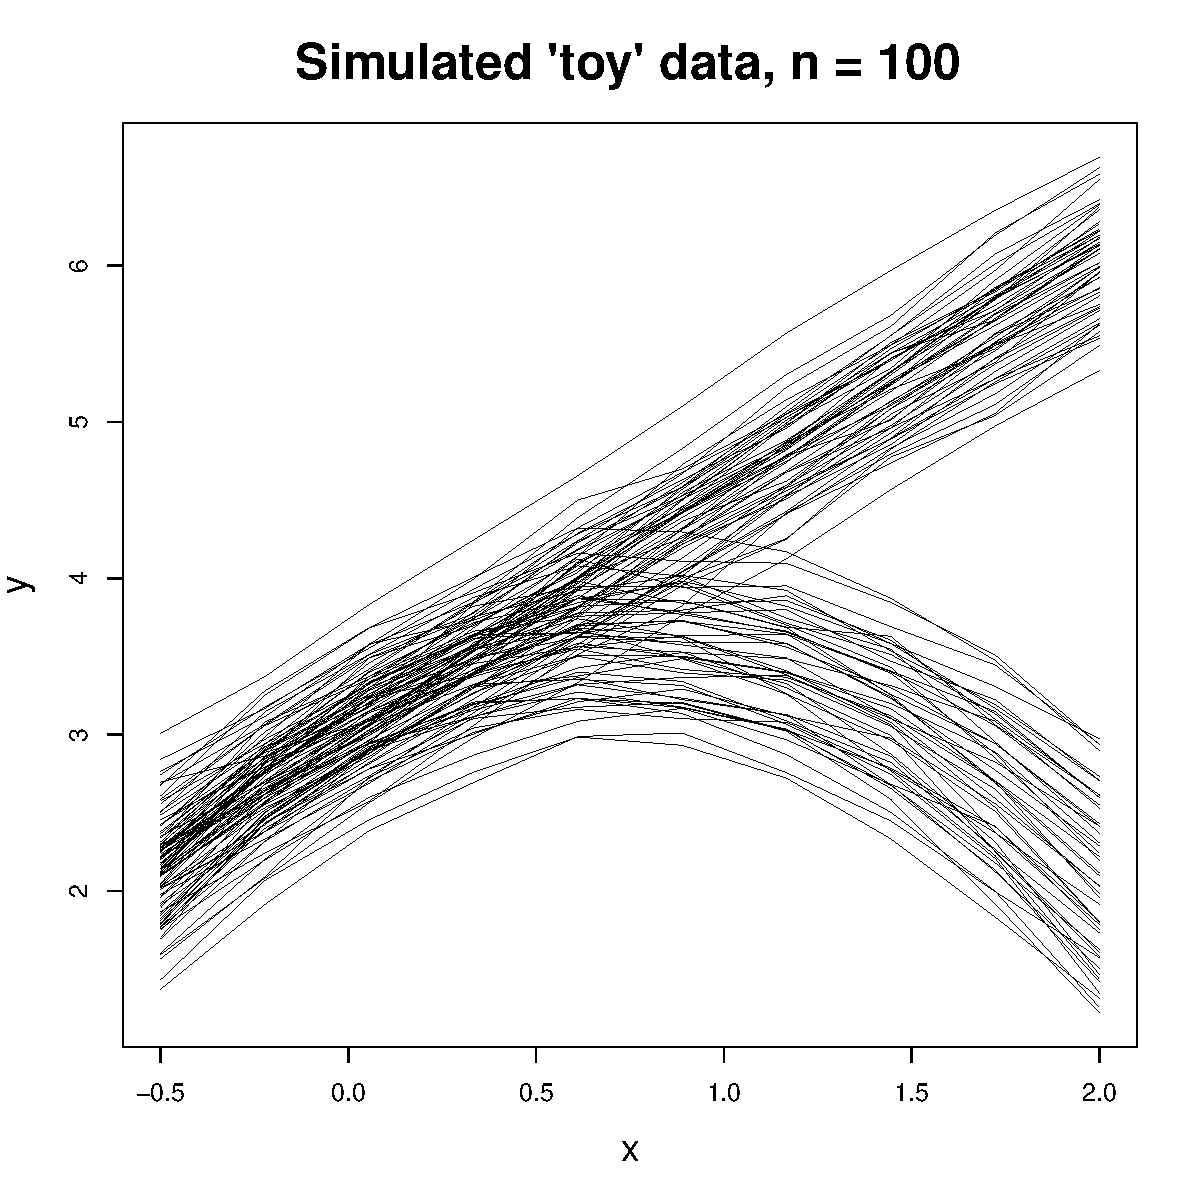
\includegraphics[scale=0.25]{../figs/toy_data.pdf}
\end{minipage}

\end{frame}

\begin{frame}
\frametitle{Data: simulated (continued)}

We use $\m{x}_1=\cdots=\m{x}_n=\m{x}$ that is a vector of $k_i=10$ equally spaced values from $-0.5$ to $2$
\bigskip

Thus we have 100 curves with random intercepts, slopes, and quadratic terms, about half of which are lines and the others are parabolas
\end{frame}

\begin{frame}
\frametitle{Parametric hierarchical model}

\begin{align*}
f(\m{y}_i|\m{x}_i,\m{\beta}_i,\tau^2) &= N_{k_i}(\m{y}_i|p(\m{x}_i, \m{\beta}_i), \tau^2\m{I}_{k_i}),~~~~~&i=1,\ldots,n \\
\m{\beta}_i &\overset{iid}\sim N(\m{\mu}, \m{\Sigma}),~~~~~&i=1,\ldots,n \\
\tau^2 &\sim IG(a_\tau, b_\tau) \\
\m{\mu} &\sim N(\m{m}, \m{S}) \\
\m{\Sigma} &\sim IW(\m{V}, d) 
\end{align*}
where $\m{\beta}_i=(\beta_{i0}, \beta_{i1}, \beta_{i2})^\top$, $p(\m{x}_i,\m{\beta}_i) = \beta_{i0}\m{1}_{k_i} + \beta_{i1}\m{x}_i + \beta_{i2}\m{x}_i^2$, and $a_\tau, b_\tau, \m{m}, \m{S}, \m{V}, d$ are specified.

\end{frame}


\begin{frame}
\frametitle{Dirichlet process mixture model for a curve}

\[ F(\m{y}_i|G,\m{x}_i, \tau^2) = \int N_{k_i}(\m{y}_i|f(\m{x}_i, \m{\theta}), \tau^2\m{I}_{k_i})dG(\m{\theta}) \]

where $f(\m{x}_i, \m{\theta})$ is a (possibly non-linear) function that maps covariates $\m{x}_i$ and latent variables $\m{\theta}$ to $\R^{k_i}$


%\begin{itemize}[label=$\cdot$]
%\item A general set of methods that allows us to obtain random samples from a target distribution
%\item In the Bayesian setting, the target distribution is the posterior distribution $p(\m{\theta}|\m{y})$
%\item MCMC is useful when directly sampling from $p(\m{\theta}|\m{y})$ is difficulty
%\item Standard MCMC methods require the parameters $\m{\theta}$ to have fixed dimension
%\end{itemize}

\end{frame}


% \begin{frame}
% \frametitle{Reversible jump MCMC}
% 
% What about when $\m{\theta}$ does not have fixed dimensions?
% \bigskip
% 
% For example, consider the normal mixture model
% \begin{align*}
% y_i &\overset{iid}\sim \sum_{j=1}^\nu \pi_j N(\phi_j, 1),~~~~~i=1,\ldots,n \\
% \nu,\m{\pi},\m{\phi} &\sim p(\nu)p(\m{\pi})p(\m{\phi}) 
% \end{align*}
% 
% Here, $\m{\theta}=(\nu,\m{\pi}, \m{\phi})$ has dimension $2\nu+1$, with random $\nu\geq 1$, and $\pi=(\pi_1,\ldots,\pi_\nu)$, $\phi=(\phi_1,\ldots,\phi_\nu)$
% 
% \end{frame}
% 
% 
% \begin{frame}
% \frametitle{Reversible jump MCMC}
% 
% Generally, we are considering a collection of $K$ models
% \begin{align*}
% \mathcal{M}_k=\{f(\cdot|\theta_k);~\theta_k\in\Theta_k\} 
% \end{align*}
% 
% We need a method that allows us to \emph{jump} from one dimension, or model, to another (i.e. moving from $\mathcal{M}_i$ to $\mathcal{M}_j$)
% 
% \end{frame}
% 
% \begin{frame}
% \frametitle{Green's (1995) algorithm}
% 
% %Green's idea is to augment $\Theta_i$ and $\Theta_j$ with artificial spaces to create a bijection between them
% %\bigskip
% 
% Let $\pi(k, \theta_k)$ denote the posterior density for model $\mathcal{M}_k$
% \bigskip
% 
% Define a $K\times K$ matrix $\{P\}_{ij} = p_{ij}\geq 0$ with row sums of 1
% \bigskip
% 
% Define a deterministic transformation function $T$ such that
% \[(\theta_j,u_j) = T_{ij}(\theta_i,u_i)\]
% where $\theta_k\in\Theta_k, u_k\sim g_k(u_k)$, for $k=\{i,j\}$ so $(\theta_i,u_i)$ has the same \emph{number} of components as $(\theta_j,u_j)$
% 
% \end{frame}
% 
% \begin{frame}
% \frametitle{Green's (1995) algorithm}
% 
% At iteration $t$, if $x^{(t)}=(i,\theta_i^{(t)})$,
% \begin{itemize}
% \item 1. Select model $\mathcal{M}_j$ with probability $p_{ij}$
% \item 2. Generate $u_{ij}\sim g_{ij}(u)$
% \item 3. Set $(\theta_j, v_{ji})=T_{ij}(\theta_i^{(t)},u_{ij})$
% \item 4. Take $\theta_j^{(t)}=\theta_j$ with probability
% \[ \min\left(\frac{\pi(j,\theta_j)}{\pi(i,\theta_i^{(t)})}\frac{p_{ji}g_{ji}(v_{ji})}{p_{ij}g_{ij}(u_{ij})}\left|\frac{\partial T_{ij}(\theta_i^{(t)},u_{ij})}{\partial(\theta_j^{(t)},u_{ij})}\right|,1\right) \]
% \item ~~~ and take $\theta_i^{(t+1)}=\theta_i^{(t)}$ otherwise
% \end{itemize}
% 
% \end{frame}
% 
% %\begin{frame}
% %\frametitle{Comments on implementation}
% %
% %Proposals are often made to another model that is similar in dimension (e.g. has only one additional or fewer parameters)
% %\bigskip
% %
% %Difficult to tune for efficient sampling: choices for $T$, $P$, $g$?
% %\bigskip
% %
% %Diagnostics for the Markov chain?
% %\bigskip
% %
% %\end{frame}
% 
% \begin{frame}
% \frametitle{References}
% 
% \citei{green1995reversible}
% \citei{richardson1997bayesian}
% \citei{robert2013monte}
% 
% \bibliography{refs}
% \bibliographystyle{asa}
% 
% \end{frame}


\end{document}
